\documentclass[11pt, a4paper]{report}
%\documentclass[11pt, a4paper]{article}

%====================== PACKAGES ======================


\usepackage[french]{babel}

\frenchbsetup{StandardLists=true}
\usepackage{enumitem}
\usepackage{pifont}

\usepackage[utf8x]{inputenc}
%\usepackage[latin1]{inputenc} % Feynman

%pour gérer les positionnement d'images
\usepackage{float}
\usepackage{amsmath}
\DeclareMathOperator{\dt}{dt}
\usepackage{graphicx}
\usepackage{tabularx}
\usepackage[colorinlistoftodos]{todonotes}
\usepackage{url}
%pour les informations sur un document compilé en PDF et les liens externes / internes
\usepackage[pdfborder=0]{hyperref}
\hypersetup{
	colorlinks = true
	}
%pour la mise en page des tableaux
\usepackage{array}
\usepackage{tabularx}
\usepackage{multirow}
\usepackage{multicol}
\setlength{\columnsep}{50pt}
%pour utiliser \floatbarrier
%\usepackage{placeins}
%\usepackage{floatrow}
%espacement entre les lignes
\usepackage{setspace}
%modifier la mise en page de l'abstract
\usepackage{abstract}
%police et mise en page (marges) du document
\usepackage[T1]{fontenc}
\usepackage[top=2cm, bottom=2cm, left=2cm, right=2cm]{geometry}
%Pour les galerie d'images
\usepackage{subfig}

\usepackage{pdfpages}
\usepackage{tikz}
%\usepackage{tikz}
\usetikzlibrary{trees}
\usetikzlibrary{decorations.pathmorphing}
\usetikzlibrary{decorations.markings}
\usetikzlibrary{decorations.pathreplacing,calligraphy}
%\usetikzlibrary{decorations}
\usetikzlibrary{angles, quotes}
\usepackage{verbatim}

\usepackage{appendix}

\usepackage{comment}

\usepackage{xcolor}


%\PreviewEnvironment{tikzpicture}
%\setlength\PreviewBorder{0pt}%

%====================== INFORMATION ET REGLES ======================

%rajouter les numérotation pour les \paragraphe et \subparagraphe
\setcounter{secnumdepth}{4}
\setcounter{tocdepth}{4}

\hypersetup{							% Information sur le document
pdfauthor = {Stephan Runigo},			% Auteurs
pdftitle = {Documentation},			% Titre du document
pdfsubject = {Documentation},		% Sujet
pdfkeywords = {Document},	% Mots-clefs
pdfstartview={FitH}}	% ajuste la page à la largeur de l'écran
%pdfcreator = {MikTeX},% Logiciel qui a crée le document
%pdfproducer = {} % Société avec produit le logiciel
%======================== DEBUT DU DOCUMENT ========================
%
\begin{document}
%
%régler l'espacement entre les lignes
\newcommand{\HRule}{\rule{\linewidth}{0.5mm}}
%
% Titre, résumé, ... %
%
\begin{titlepage}
%
~\\[1cm]

\begin{center}
%\includegraphics[scale=0.5]{./presentation/chambreABulle}
\end{center}

\textsc{\Large }\\[0.5cm]

% Title \\[0.4cm]
\HRule

\begin{center}
{\huge \bfseries  La causalité\\
%titre 2\\[0.4cm]
 }
\end{center}

\HRule \\[1.5cm]

\begin{center}
%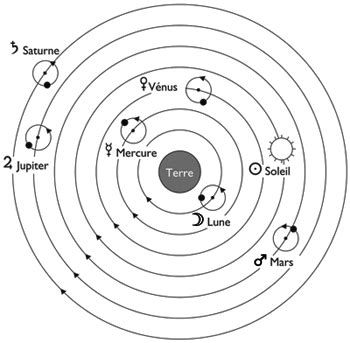
\includegraphics[scale=0.3]{./presentation/ptoleme}
\end{center}

\begin{center}
%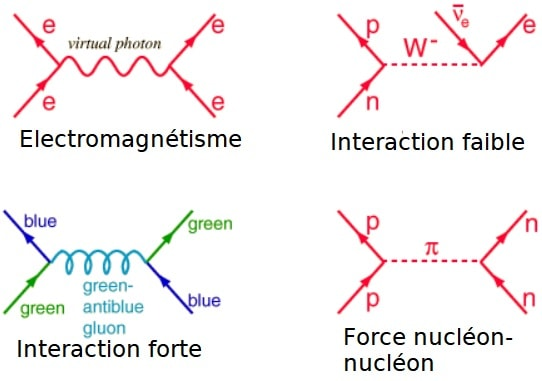
\includegraphics[scale=0.3]{./presentation/diagrammesInteractions}
\end{center}


% Author and supervisor
\begin{minipage}{0.4\textwidth}
\begin{flushleft} \large
%\emph{Auteur:}\\
%Stephan \textsc{Runigo}
\end{flushleft}
\end{minipage}
\begin{minipage}{0.4\textwidth}
\begin{flushright} \large
\emph{Auteur:}\\
Stephan \textsc{Runigo}
\end{flushright}
\end{minipage}

\vfill

% Bottom of the page
{\large \today}

\end{titlepage}

\newpage
\begin{center}
\Large
Résumé
\normalsize
\end{center}
\vspace{3cm}
\begin{itemize}[leftmargin=1cm, label=\ding{32}, itemsep=21pt]
\item {\bf Objet : } Souvenir des questions posés.
\item {\bf Contenu : } Définition, analyse, reflexion.
\item {\bf Public concerné : } Interressé à la question de l'âme.
\end{itemize}

\vspace{3cm}



\vspace{3cm}


%

%
% Table des matières
\tableofcontents
\thispagestyle{empty}
\setcounter{page}{0}
%
%espacement entre les lignes des tableaux
\renewcommand{\arraystretch}{1.5}
%
%====================== INCLUSION DES PARTIES ======================
%
~
\thispagestyle{empty}
%recommencer la numérotation des pages à "1"
\setcounter{page}{0}
\newpage
%
%\chapter{Histoire}
%

\section{Vocabulaire}
\newpage
\subsection{cause}
	\begin{itemize}[leftmargin=1cm, label=\ding{32}, itemsep=11pt]

\ib{Causalité} — \si{Épist.} Rapport de cause*
à effet. — Principe de causalité :
« Tout a une cause et, dans les
mêmes conditions, la même cause
est suivie du même effet. »

\ib{Cause} — \si{Méta.} {\bf 1.} Force$^2$ productrice,
engendrant l'effet et se prolongeant
en lui. {\it cf.} {\it Efficace}* et {\it Occasionnelle}*. — \si{Épist.} {\bf 2.} Antécédent$^1$
constant (Hume) et inconditionnel
(J. S. Mill). — {\bf 3.} Phénomène lié au
phénomène considéré par une relation fonctionnelle : « La cause n’est
jamais vraiment empirique » (Bachelard) $->$ {\it Dans la science}, l'explication par les forces productrices
(sens 1) fait place de plus en plus à
l’explication par les relations fonctionnelles (sens 3). Aussi, tandis
que F. Bacon disait que « savoir
vraiment, c’est savoir par les causes »
(sens 2), A. Comte a pu écrire
(Cours, I) que la science renonce à
la recherche des causes (sens 1), ce
qui est d'ailleurs auj. discuté.

—— \si{Hist.} {\bf 4.} {\it Aristote} distingue
4 espèces de causes : a) la cause matérielle ({\it p. e.} dans une statue, la
matière dont elle est faite); — b) la
cause formelle (la figure que la statue
représente; {\it cf.} Formel); — c) la
cause efficiente, {\it i. e.} la cause au sens 1
(le sculpteur); — d) la cause finale$^1$
(le but : désir de la gloire ou du gain,
visé par le sculpteur).

— \si{Méta.} {\bf 5.} Cause première : voir
Premier$^4$.

	\end{itemize}
\subsection{effet}
	\begin{itemize}[leftmargin=1cm, label=\ding{32}, itemsep=11pt]

\ib{Effet} — \si{Épist.} {\bf 1.} Phénomène considéré comme produit par
une cause efficiente*. — \si{Psycho.} {\bf 2.} Loi de
l'{\it effet} : celle qui pose que « toutes
% 62
choses égales d’ailleurs, une réponse
est renforcée par le succès, affaiblie,
éliminée, ou remplacée à la suite de l'échec » (Lagache).

\ib{Efficace} — \si{Méta.} Qui produit réellement son effet : « Cause efficace »
({\it opp.} « occasionnelle* »).

\ib{Efficience} — \si{Épist.} {\bf 1.} ({\it Opp.} : {\it finalité}*).
Causalité efficiente* : « La
science ne peut s'intéresser à la finalité qu'après avoir épuisé tout son
effort dans la découverte de l’efficience » (F. Houssay).

— \si{Vulg.} {\bf 2.} [Angl. : {\it efficiency}].
Rendement, effet utile : « Le pragmatisme* est une théorie de
l’efficience de la connaissance. »

\ib{Efficiente (Cause)} — Celle qui « produit » l'effet (cf.
{\it efficace}*). Cette expression s'emploie  {\it auj.} comme
syn. de {\it cause}* tout court (aux
sens 1, 2 et même 3), et par {\it opp.}
à {\it cause finale} (cf. {\it Cause}$^4$). {\it Chez
Aristote}, au ctr., la cause efficiente
se subordonne à la cause finale :
c’est « l’activité qui sort du fond
même de l’être et tend à réaliser la fin » (Goblot).

	\end{itemize}

\subsection{hasard}
	\begin{itemize}[leftmargin=1cm, label=\ding{32}, itemsep=11pt]

\ib{Hasard} — \si{Vulg.} Ce qui n’est pas prévisible : {\bf 1.} soit qu’on
suppose dans les choses une indétermination$^2$ radicale ; — {\bf 2.} soit
qu'il s'agisse d'événements si complexes (cf. {\it Fortuit}*) qu’on ne puisse
en connaître toutes les conditions : « Il n’y a pas incompatibilité entre le
rôle de ce que nous appelons le hasard et l’établissement de lois
scientifiques » (Borel) ; — {\bf 3.} soit qu’on ignore le déterminisme$^1$ du
phénomène ; — {\bf 4.} soit que, se plaçant au point de vue de la finalité*,
on n’en aperçoive
% 86
pas les raisons d’être : « Ce qui est hasard à l’égard des hommes
est dessein à l'égard de Dieu » (Bossuet). $->$ Terme très équivoque.

	\end{itemize}

\newpage
\section{Solution ontologique et solution législative}

%https://www.sciencepresse.qc.ca/blogue/cerveau-niveaux/2019/05/14/faire-quand-survient-ecart-entre-theorie-observation
%https://fr.linkedin.com/pulse/r%C3%A9solution-ontologique-ou-l%C3%A9gislative-deli%C3%A8ge-builder-of-influencers
%https://forums.futura-sciences.com/archives/822692-solution-ontologique-legislative.html
%https://www.researchgate.net/publication/360773689_La_matiere_noire_une_enigme_de_la_cosmologie_contemporaine

L'observation du mouvement des planètes de notre système solaire s'est affinée au cours des temps. Les observations anciennes ont conduit à la mécanique aristotélicienne : les planètes ont un mouvement circulaire autour de la terre immobile. Des observations plus rigoureuse ont montré des mouvements plus compliqué que de simple cercle : cela à conduit à la théorie des épicycles.

Dix siècles plus tard, La révolution copernicienne conduit à l'invention de la mécanique newtonienne, qui s'impose face à la mécanique aristotélicienne.
%Face à des observations précises, une loi plus générale

La mécanique newtonienne permet de prédir les trajectoires des planètes de façon plus précise que la mécanique aristotélicienne.

Mais l'histoire ne s'arrète pas là. Des observations toujours plus précise vont conduire à découvrir que les trajectoires d'Uranus et de Mercure diffère des trajectoires calculées à partir de la nouvelle mécanique. Afin d'expliquer ces différences, des solutions vont finir par s'imposer.

Dans le cas d'Uranus, la solution va aboutir à la découverte d'une nouvelle planète : Neptune. Dans le cas de Mercure, la solution va aboutir à la découverte d'une nouvelle théorie : la relativité générale.

%La mécanique newtonienne permet de déduire la trajectoire des planètes de notre système solaire.

\newpage
\section{Le temps}

Les équations de newton font intervenir une variable. Newton appelera cette variable {\it temps}, concept existant se rapprochant le plus (pour Newton) de la variable introduite dans les équations.

\newpage
\section{Les quarks}

Les quarks sont les constituants des hadrons (proton, neutron, ...). Un neutron, comme un proton, est constitué de trois quark. Les quarks sont soumis à la force forte. Cette force, décrite dans la seconde moitié du {\footnotesize XX}$^\text{e}$ s., maintient les quarks entre eux.

Comme la force gravitationnelle maintient les planètes autour du soleil, la force électromagnétique maintient les électrons autour du noyau, la force forte maintient les quarks dans les protons et les neutrons. la force forte maintient également les protons et les neutrons dans les noyaux.

L'invention (la découverte) de la force forte a nécessité de baptiser de nouvelles grandeurs physiques.


\begin{center}
{\large\begin{tabular}{ccccc}
{\sf Interaction} & : & {\bf gravitationnelle} & {\bf électromagnétique} & {\bf forte} \\
{\sf remarque} & : & toujours attractive & attractive ou répulsive & toujours attractive ? \\
{\sf grandeur} & : & {\bf masse gravitationnelle} & {\bf charge électrique} & {\bf saveur} \\
{\sf remarque} & : & toujours positive & positive ou négative & 6 saveurs \\
\end{tabular}}
\end{center}


\newpage
\chapter{Formulaire}
\subsection{Mécanique analytique}

Action S et lagrangien L

Principe

\[
S = \int_{t_1}^{t_2} L(q_i, \dot{q}_i, t)dt \ \ \ \ \ \ \text{est extrémale}
\]

L'invariance du lagrangien par translation temporelle entraine le théorème :

\[
E \ \text{est une constante du mouvement}
\]

\subsection{Thermodynamique}

Énergie U, entropie S, température T, chaleur Q, travail W,  pression P, volume V

Principes
\[
dU = \delta Q + \delta W \ \ \ \ \ \ dS = \frac{\delta Q}{T}
\]
Théorème TdS
\[
dU = TdS - pdV
\]

\subsection{Quantique}
L'énergie est une observable, dans un système isolé,
\[
\mc{H}|\psi(x,t)\rangle=E|\psi(x,t)\rangle
\]


\[
\mc{H} = -i\hbar\frac{\partial}{\partial t} \ \ \ \ \ \ \ \mc{P} = i\hbar\frac{\partial}{\partial x}
\]

\newpage
\section{Onde et particule}
La physique classique (De Newton à Maxwell) distingue les phénomènes ondulatoires des phénomènes particulaires. Une onde se propage, s'étend, est susceptible d'interférence, une particule conserve sa forme, est susceptible d'en choquer une autre, suit une trajectoire.

\begin{center}
{\sf Figure : diffraction, interférence, choc, trajectoire.}
\end{center}

La nouvelle physique (quantique) unifie ces phénomènes, le nouveau paradigme ne distingue plus les ondes des particules, il n'y a que des quantons (ou des champs dans les théories les plus récentes $\to$ Feynmann).




%
%
%%%%%%%%%%%%%%%%%%%%%
\chapter{Paradigmes}
%%%%%%%%%%%%%%%%%%%%%

\section{Mécanique Newtoniennne}
%
La trajectoire d'un corps est décrite par ses coordonnées évoluant au cours du temps, obéissant au lois de la mécanique.
%
\section{Mécanique quantique}

L'évolution au cours du temps d'un quanton est décrite par sa fonction d'onde donnant l'amplitude de probabilité de mesurer ce quanton (de l'observer). La fonction d'onde evolue suivant l'équation de Schrödinger.

\section{Théorie quantique des champs}

Les différents champs échangent de l'énergie entre eux de manière quantique.

%%%%%%%%%%%%%%%%%%%%%%%%%%%%%%%%%%%%%%%%%%%%%%%%%%%%%%%%%%%%%%%%%%%%%%%%%%%%%%%%%%%%%

%
%
%%%%%%%%%%%%%%%%%%%%%
\section{Champs quantiques}
%%%%%%%%%%%%%%%%%%%%%
%
Une particule élémentaire est décrite par une fonction d'onde. Un ensemble de particules élémentaires identiques sont décrites par la superposition, la somme, des fonctions d'ondes individuelles. Ce champ total, pour un type de particule est à même de décrire l'ensemble de ces particules.

Ainsi, l'ensemble des électrons est décrit par le champ électron, l'ensemble des photons est décrit par le champ photon. Ces deux champs sont présent dans l'espace temps, la détection d'un photon ou d'un électron est due à un échange élémentaire d'énergie entre ces deux champs.

Lorsqu'un photon se matérialise en une paire électron-positron : un transfert d'énergie s'oppère du champ photon vers le champ électron. Lorsqu'un électron rencontre un positron, ils s'anihilent donnant un photon :  un transfert d'énergie s'oppère du champ électron vers le champ photon.

Une particule élémentaire peut alors être considérée comme l'évènement : transfert d'énergie entre deux champs quantique, la matière classique ne serait donc que la manifestation de ces évenements.

Les évènement de transfert d'énergie entre deux champs quantique caractérise le \textsf{\textit {couplage}} entre les champs.

L'existence (ou la détection) de la force électrique entre un électron et un proton serait la signature du couplage entre le champ électron et le champ photon d'une part et du couplage entre le champ proton et le champ photon. Le champ photon est le médiateur de la force électrique entre les particules chargées.
%%%%%%%%%%%%%%%%%%%%%%%%%%%%%%%%%%%%%%%%%%%%%%%%%%%%%%%%%%%%%%%%%%%%%%%%

%
%
%%%%%%%%%%%%%%%%%%%%%
\chapter{Observables}
%%%%%%%%%%%%%%%%%%%%% de l'antiquité à la renaissance
% \textsc{} \textbf{\textit {}} \textsf{\textit {}}
% {\bf }{\it }{\bf --} « » “” ° {\footnotesize X}$^\text{e}$
Extrait d'{\it histoire du principe de relativité} de {\sc Tonnelat}.
%\vfill
%

% Author and supervisor
\begin{minipage}{0.5\textwidth}
\begin{flushleft} \large
%
\end{flushleft}
\end{minipage}
\begin{minipage}{0.5\textwidth}
%\begin{flushright}
Toute philosophie de la nature est seulement de
l’anthropomorphisme. L’homme pour sauvegarder son
unité personnelle répartit sur toute chose ce qu’il n’est pas.

\hfill {\sc W. G{\oe}the}

%\end{flushright}
\end{minipage}


\section{Introduction}
%{\bf }{\bf --}{\it } {\footnotesize XIX}$^\text{e}$
%CHAPITRE PREMIER

%RELATIVISME ET RELATIVITÉ
%DE L'ANTIQUITÉ A LA RENAISSANCE

L'idée de Relativité, comme la plupart des concepts de la Physique
moderne est une notion vivante dont le sens s’est précisé petit à petit
au cours d’un développement tourmenté et incertain. Au risque de
décevoir certains spécialistes, nous affirmerons donc qu’il n’existe pas
une authentique et imperfectible Relativité dont nous nous proposerions
de rechercher l’esquisse dans les premiers développements des théories
scientifiques. Aucune ébauche imparfaite mais prometteuse, n’attend sous
le voile des ignorances et des préjugés une sorte d’investiture. Cette idée
même est antirelativiste.

La Relativité générale, nous le verrons, est une théorie physique, celle
des phénomènes de gravitation; la Relativité Restreinte constitue une
nouvelle cinématique; la Relativité, sans autre qualificatif, est presque
un état d’esprit souvent confondu avec l’exigence même d’une explication
 rationnelle dans les Sciences.

Bien loin d’être « instinctive », la notion de Relativité, comme celle
d'inertie qui lui est souvent associée, a demandé un renversement des
évidences, une « mutation de l’intellect humain ». Ce qui était inconcevable
devient naturel, puis familier. Née dans la confusion de l’aristotélisme
finissant, rénovée par les contradictions attachées à un insaisissable
éther, l’idée de Relativité semble chaque fois liée davantage à ce
qui la suit qu’à ce qui la précède. Vision novatrice, elle éclaire son propre
chemin et même, dans une large mesure, en définit les méandres et en
détermine l’approfondissement.


%\newpage
\section{Des observables aux grandeurs physiques,
des phénomènes à la loi}
%{\bf }{\bf --}{\it } {\footnotesize XIX}$^\text{e}$
%14 M. À. TONNELAT
%\footnote{}size[]
%1.

L'observation immédiate nous introduit au cœur d’une situation
complexe. L'univers est « tout d’une pièce, comme un océan »
%{\footnotesize [{\sc Leibniz}, {\it Opera Philosophica}, éd. Erdmann, p. 506]}.
{\footnotesize [{\sc Leibniz}, {\it Opera Philosophica}]}.
Les ressemblances et les répétitions que nous pouvons y discerner sont inextricablement
mêlées à des caractères particuliers et changeants. « Si nos
faces n’étaient semblables,
% écrivait Montaigne, 
%{\footnotesize [{\sc Montaigne}, {\it Essais}, Paris, Flammarion, vol. IV, p. 194]}
on ne saurait discerner
l’homme de la bête ; si elles n’étaient dissemblables on ne saurait discerner
l’homme de l’homme. »
{\footnotesize [{\sc Montaigne}, {\it Essais}]}
La perception puis l’expérimentation nous
livrent un résultat brut, complexe, mais somme toute inéluctable : les
\textbf{\textit {observables}}{\it }. C’est l’enchaînement entre les diverses observables qui constitue
le \textbf{\textit {phénomène}}{\it }. Au sens étymologique, le phénomène s’identifie aux
apparences. Rien {\it d’illusoire ou de fallacieux ne doit être associé à ce
qualificatif d’« apparent »}. Il signifie tout simplement qu’observables et
phénomènes sont liés, par définition, à l’observation et à ses modalités.
Ils en demeurent nécessairement tributaires; ils n’ont de sens que par
rapport à l’observateur même et à son état de mouvement.

C’est un lent travail de systématisation et de discernement qui conduit
de l’idée immédiate, mais fragmentaire, d’observable à la notion
élaborée, mais synthétique, de grandeur physique. Partant de la perception
immédiate du phénomène, il mène à l’enchaînement nécessaire que
constitue la loi.

Ce travail consiste à construire l’objet à partir de ses traces dans
l'expérience de l’observateur, c’est-à-dire à partir d’observables et de
mesures relatives. La correspondance peut sembler très simple dans
certains cas. Par exemple, la donnée du diamètre apparent du soleil
jointe à la connaissance de la distance qui nous sépare de celui-ci permettra
de déterminer les dimensions « vraies » du soleil. Ainsi, au sens
de la Mécanique classique, un jeu d’observables (dépendant par définition
des modalités de l’observation) peut être équivalent à des données
sur les dimensions « intrinsèques » de l’objet
%{\footnotesize [Nous assimilerons pour le moment « objet » et grandeur intrinsèque. Ce
%rapprochement est sans ambiguïté dans la physique classique]}.
Néanmoins, pour être
capable de reconstruire l’objet sans ambiguïté, il faut être assuré de
disposer d’un jeu « complet » d’observables. Une assurance trop vite
%HISTOIRE DU PRINCIPE DE RELATIVITÉ 15
acquise engendre les prétentions des sophistes. Elle entraîne la Mécanique
classique elle-même vers des illusions que devra dissiper la
Relativité Restreinte.

Même à ce stade, le passage de l’observable à l’objet s’accompagne
d’inévitables critères théoriques. Ils interviennent {\it a fortiori} dès que
l’« objet » est lié à des manifestations plus indirectes. La hauteur de la
colonne barométrique est une observable qui manifeste un « objet » très
élaboré : la pression atmosphérique.

Ainsi la construction d’un objet constitue toujours une idéalisation.
Mais la solidité et la nécessité de celle-ci présente d’incontestables privilèges :
l’objet est indépendant de l’observateur et de son mouvement. Il
est affranchi du {\it hic} et du {\it nunc}
{\footnotesize [de l'ici et du maintenant, n.d.n]}
inhérents à toute observation.

Les observables et le phénomène qui les relie partagent la solidité
mais aussi les vicissitudes d’une situation de fait; l’objet de la loi physique
bénéficie du prestige mais aussi de la fragilité d’une situation de
droit. Il peut servir de thème explicatif pour ordonner l’ensemble de
l’expérience sensible
%{\footnotesize [L'idée de grandeur physique est utilisée ici dans le sens classique, et non dans
%l’acception assez particulière de la Mécanique Quantique. En Mécanique quantique
%l’objet se réduit à des données statistiques et n’est plus localisable dans
%l’espace-temps si son état de mouvement est bien déterminé.
%Nous nous limiterons, dans tout ce qui suit, aux conceptions purement classiques]}
;
il constitue un élément de l’édifice scientifique.

La distinction entre {\it observable} et {\it grandeur physique} nous semble
essentielle pour interpréter les progrès de l’esprit relativiste. Insistons
sur le fait qu’elle est entièrement indépendante d’une ontologie sous-jacente.
%{\footnotesize [Nous éviterons de lier univoquement et de façon exclusive le critère de
%« réalité » qui, pour un physicien, comporte en fait un jugement de valeur soit
%à la notion d’{\it observable} sous prétexte qu’il s’agit d’une donnée brute et affranchie
%de toute élaboration théorique (ce qui est d’ailleurs inexact), soit, au contraire,
%à la notion d’{\it objet} en arguant du fait qu’elle est affranchie des contingences et des
%modalités inhérentes à toute expérience particulière.
%Attacher le critère de « réalité » à l’un ou bien à l’autre de ces points de vue
%c’est déjà prendre parti sur la signification de la Relativité.]}
Ainsi, pour Ptolémée, le soleil mobile autour de la terre
entraînant son cortège d’astres errants constituait une grandeur physique
authentique ou, si l’on préfère, la représentation qui rendait compte de
l’ensemble de l’expérience sensible et des mesures de son époque. Il se
substitue à la perception de cet objet minuscule, chaque jour nouveau,
qui apparaît à l'Orient. Une grandeur physique est donc toujours {\it objective}
en ce sens qu’elle satisfait — même de façon embryonnaire — un
ensemble de lois, qu’elle groupe — même pour un temps limité — une
série d’observations. On peut, sans inconvénient, réduire ces « idéalisations »
%TONNELAT. — Histoire du principe de relativité. 2
%16 M. À. TONNELAT
à de purs jeux d’ombres : il suffira pour qu’elles deviennent
objets de physique, que ces ombres satisfassent l’optique d’Euclide.
A cette condition, mais à cette condition seulement, la caverne des
magiciens devient laboratoire.

Par définition même, les observables et leur association en cohortes
de phénomènes constituent des données immédiates; elles s’intègrent
à une situation d’ensemble qui comprend, en particulier, les conditions
de l’observation. Nous appellerons {\it relativisme} cette dépendance vis-à-vis
de l’observation ou, si l’on préfère, cette subordination à l’observateur.
{\it Une observable, un phénomène constituent des données essentiellement relatives.
Il n’y aurait pas plus de sens à nier le relativisme d’une observable ou
d’un phénomène qu’à contester leur existence.}

Au contraire, la {\it grandeur} ou la {\it loi physique} constitue, par construction,
des {\it absolus} en ce sens qu’{\it elles sont indépendantes des modalités de
l'observation}. Bien entendu, cet absolu est pratiquement fonction de la
science du moment et de l’ensemble des connaissances de l’époque.
Néanmoins, nier l’existence de cet objet, de cette loi, ou plutôt l’identifier
aux impressions fluctuantes d’un instant c’est abolir sa raison d’être,
c’est construire, à côté de la perception, un rêve capricieux et incohérent,
un rêve inutile.

Cette assimilation fallacieuse de l’objet à l’observable, de la loi au
phénomène est cependant une tentation de tous les temps. Un Relativisme
philosophique étend indûment à l’objet, à la loi, cette subordination à
la perception immédiate, ce « relativisme » scientifique qui caractérise
l’observable et le phénomène.


%{\footnotesize [Nous assimilerons pour le moment « objet » et grandeur intrinsèque. Ce
%rapprochement est sans ambiguïté dans la physique classique]}.

\newpage
%\section{Le Relativisme des Sophistes}
%{\bf }{\bf --}{\it } {\footnotesize XIX}$^\text{e}$

« L'homme est la mesure de toutes choses affirmait déjà Protagoras
d’Abdère
%{\footnotesize [XÉNOPHANE, Fragment 1]};
de celles qui sont, en tant qu’elles sont, de celles qui ne
sont pas en tant qu’elles ne sont pas. » C’est ainsi que, pour Xénophane,
les astres s’allument à l’Orient, s’éteignent à l’Occident. Leur vraie
grandeur est celle que manifeste l’observation immédiate et le soleil,
« chaque jour nouveau »
%{\footnotesize [PROTAGORAS, Fragment 6]}
a « la largeur d’un pied d’homme ».
%{\footnotesize [XÉNOPHANE, Fragment 3]}.

%17
Ces affirmations naïves caractérisent un Relativisme intégral, naturel
tant qu’il s’agit d’observables arbitraires dont l’enchaînement constitue
un phénomène, entièrement stérile s’il est question de grandeurs intrinsèques
liées par une loi. Les opinions de Xénophane conduisent alors
inévitablement au sophisme de Gorgias : rien ne peut être connu et toute
Science est parfaitement vaine et inutile.

Des opinions parentes du sophisme mais infiniment plus nuancées
ont des résurgences dans un certain humanisme de tous les temps. Elles
apparaissent alors comme une sorte de tentation qui voudrait opposer
les desseins d’une Science sèche ou trop ambitieuse au devenir harmonieux
de l’homme. Ceux-là doivent alors être subordonnés à celui-ci dès
que l’on veut jouer les uns contre l’autre.

Les enseignements de Socrate ne sont pas exempts d’une telle illusion;
le réquisitoire antinewtonien de Gœthe n’en est pas non plus dépourvu.
Au {\footnotesize XVII}$^\text{e}$ siècle, on soupçonnera les lunettes de véhiculer des visions
illusoires ; bien plus tard, on accusera le prisme de dénaturer la lumière
qui baignait la campagne italienne, la Science de défigurer une instructive
et intuitive vérité : « Toute philosophie de la nature, écrit Gœthe, est
seulement de l’anthropomorphisme : l’homme, pour sauvegarder son
unité personnelle, répartit sur toute chose ce qu’il n’est pas. Retranscrit
dans son unité, ceci ne fait qu’un avec lui-même. »

En fait, le Relativisme intégral est une retombée de l’Humanisme. Au
contraire, le développement authentique de celui-ci ne peut se réaliser
sans une abdication qui dans la Science, dans le style, dans l’Art permet
de se servir du particulier puis de le dépasser pour retrouver ainsi ce qui
peut être commun à tous.

Il n’est pas rare, nous l’avons dit, de constater que le Relativisme de
Protagoras a été confondu avec les prémisses de la théorie d’Einstein
dont le sens est diamétralement opposé. On a cru que l’homme ou, plus
exactement, que l’observateur était la mesure de toute chose, que les
objets, à l’instar des phénomènes, devenaient inféodés à son temps, à son
espace, à son système de référence. Se refusant à distinguer les observables
— qui, bien entendu, dépendent de l’observation — des structures intrinsèques
qu’elles permettent de mettre en évidence, on s’est refusé à reconnaître
l’invariance de celles-ci qui se traduit par la covariance de la loi.

C’est ainsi que J. Petzoldt
%{\footnotesize [J. PETZOLDT, Die Stellung der Relativitätstheorie, p. 15]}
estimant que la Relativité est un corollaire
du positivisme de Mach, rattache l’une et l’autre au subjectivisme de
%18
Protagoras « Ç’a été le malheur de l’humanité, écrit-il, que l'opinion saine
de ce phisolosophe n’ait pu prévaloir contre les doctrines de Platon et
d’Aristote ; le Moyen Age lui eût été épargné ».

Bien au contraire, le Principe de Relativité fut de tout temps, comme
le remarque Meyerson,
%{\footnotesize[E. MEYERSON, La déduction Relativiste, p. 68)]}
celui de la non-relativité du réel ». Il se situe
dans la ligne de cette « émancipation anthropomorphique » que Planck
reconnaît comme l’évolution nécessaire de toute théorie physique.
Néanmoins, ce passage à l’« objectif » ne doit pas se confondre avec une
assimilation passive aux données particulières des apparences immédiates.


%\newpage
%\section{Mouvement relatif. Mouvement absolu}
%{\bf }{\bf --}{\it } {\footnotesize XIX}$^\text{e}$

\subsection{Mouvement relatif}
Les observables les plus immédiates que manifeste
l’expérience se rapportent à la position et aux mouvements des corps.
Dire qu’il s’agit d’observables signifie ipso facto que ces notions se
rapportent à l’observateur \footnote{Dans cet ouvrage nous utiliserons à maintes reprises le mot « observateur ».
I ne doit pas nous faire illusion. Ce terme ne recouvre pas l’idée d’un être pensant
susceptible d’ériger ses perceptions en opinions subjectives, de les déformer éventuellement.

L’observateur est le support désincarné, mais cependant matériel, auquel est lié
un système de référence et, avec celui-ci, une possibilité de mesure. L’observateur
est muni de règles et d’horloges mais dénué de passion. Il effectue des mesures à
l’aide de ses instruments, il observe des coïncidences. Son « humanité » s’arrête là.

Nous emploierons toujours le mot « observateur » dans ce sens qui ne comporte
ni subjectivisme, ni jugement de valeur. Nous ne reviendrons plus sur l’absence
de tout caractère anthropomorphique de tels observateurs.}. Il ne s’agit aucunement des impressions
purement subjectives de celui-ci. Pour éviter tout abus de langage, nous
dirons que ces notions traduisent immédiatement les mesures réalisables
dans un système de référence lié à l’observateur.

Le célèbre exemple du mouvement d’une bille sur le pont d’un
bateau en marche, mouvement différent suivant qu’on l’observe du pont
ou de la rive, ne donne lieu à aucune discussion tant qu'il s’agit des
apparences pures et simples de ce mouvement. Les notions de vitesse
relative, de mouvement relatif inhérentes à toute mesure n’ont jamais
prêté à discussion, que le physicien se nomme Aristote, Galilée ou Einstein.
La description d’un mouvement « relatif » est réalisée par des expériences
portant d’un système sur l’autre.

Il va de soi que ce mouvement relatif (évaluation des coordonnées du
point « mobile » dans le système « fixe ») s’accompagne d’une totale
réciprocité.


HISTOIRE DU PRINCIPE DE RELATIVITÉ 19

Il est plus important de souligner que la détermination d’un mouvement
relatif ne peut s’effectuer que par rapport à un système de référence
matériel. 1 exige l’intervention d’un « solide de référence ». En effet,
toute expérience portant d’un système sur l’autre exige une interaction
par l’intermédiaire d’un signal lumineux ou d’un mobile matériel. C’est
en ce sens matérialiste que doit être comprise la notion de mouvement
relatif.

\subsection{Mouvement absolu}

Le mouvement relatif se rapporte à un repère arbitraire. Il ne peut
nous renseigner sur le lieu absolu du mobile ni sur la direction intrinsèque
de son mouvement. On peut penser — et telle a été pendant
longtemps l’opinion admise — que le mouvement relatif ne pouvait
exprimer qu’une apparence cinématique. Il manifesterait — sans épuiser
sa nature — un véritable changement de lieu qui aurait constitué le
mouvement absolu.

« Tout d’abord, écrit Maxwell \footnote{MaxweLL, Matter and Motion, Préface.}, nous pouvions penser que notre
condition d’êtres conscients impliquait, comme éléments essentiels du
savoir, la connaissance absolue du lieu dans lequel nous nous trouvions
et de la direction de notre mouvement. Mais cette opinion qui était
indubitablement celle de nombreux Sages de l’Antiquité a disparu de
plus en plus des conceptions du physicien. Dans l’espace, il n’existe pas
de bornes kilométriques ; une portion d’espace est exactement semblable
à une autre, de sorte que nous ne pouvons pas savoir où nous sommes.
Nous nous trouvons dans une mer sans vagues et sans étoiles, sans
boussole ni soleil, sans vent ni marée, et nous ne pouvons dire dans
quelle direction nous allons. Nous n’avons pas de données que nous
pourrions exploiter pour faire un calcul. Nous pouvons, bien entendu,
déterminer notre mouvement par comparaisons avec les corps voisins
mais nous ignorons ce qu’est le mouvement de ces corps dans l’espace. »

La détermination du mouvement absolu dans l’espace absolu ne peut
donc recevoir, selon certains auteurs, qu’une solution « analogue à celle
du mouvement perpétuel et de la quadrature du cercle » \footnote{CassIReR, Einstein’s theory of Relativity, Dover Public. 1953, p. 408.}. Il fallait
transformer cet « aspect négatif », cette « limitation du savoir » en un
principe de connaissance. L’histoire de la Relativité est celle de cette
acquisition.


%\newpage
%\subsection{La Physique d’Aristote et la notion de mouvement absolu}
%{\bf }{\bf --}{\it } {\footnotesize XIX}$^\text{e}$
%20

La physique d’Aristote se présente comme une entreprise beaucoup
trop structurée pour ne pas avoir aperçu, comme on le croit trop souvent,
que tout mouvement local devait être à la fois relatif et absolu. Il est
relatif parce que la retranscription d’un mouvement quelconque dans
l’expérience d’un autre observateur procède d’une comparaison et n’a
aucun sens intrinsèque. Il est absolu parce que cet indéniable relativisme
de fait n’atteint pas l’essence du mouvement qui est altération et changement.

Cette affirmation nous apparaît comme un postulat gratuit dans le
domaine de notre physique. Par contre, elle découle nécessairement de
la métaphysique d’Aristote. En effet, sa Mécanique est accrochée à la
conception du premier moteur. Elle en retire son caractère essentiel. Les
attributs du mouvement ne peuvent donc constituer une convention
accessoire ni un postulat surajouté.

Une description authentique du mouvement requiert ainsi un terme
absolument immobile, origine ou aboutissement. Le mouvement d’une
pierre est un phénomène original qui possède sa finalité propre. On
pourrait dire qu’il est suspendu à la physique du cosmos tout entier.
La notion expérimentale de mouvement relatif, même s’il s’agit de déplacement
rectiligne et uniforme, n’épuise donc aucunement l’essence du
mouvement.

En admettant les conceptions aristotéliciennes, le caractère absolu du
mouvement n’est pas forcément lié à l’apparition de manifestations qui
traduiraient sa présence par des caractères secondaires mais, somme
toute, accessoires. Les « effets physiques du mouvement », inséparables
de la dynamique newtonienne, ont une interprétation bien différente
dans la physique d’Aristote. L’état de mouvement est intrinsèquement
différent de l’état de repos comme l’état solide est différent de l’état
liquide. Tout changement (accélération, décélération) dans le régime du
mouvement, tout « effet » dont la nature est étrangère au mouvement
lui-même, manifeste l’intervention de contraintes. Pourtant, les actions
violentes ne sont nullement nécessaires pour définir le mouvement
absolu. Celui-ci se reconnaît plutôt dans une unité d'intention qui donne
à l’expérience une interprétation quasi-organique. Ainsi un voyageur
contemple un paysage fugitif et mouvant qu’il « sait » pourtant immobile,
%21
non pas en raison des accélérations au départ et à l’arrivée, mais par le
fait que départ et arrivée constituent le début et la fin d’une intention
que régit une finalité. Tout mouvement implique cette intention, cette
finalité qui dépasse à vrai dire une physique du cosmos, mais dont la
cinématique (vitesse relative) laisse échapper la véritable nature.

Au cours de cette longue période qui va s’achever à la Renaissance,
avec les travaux de Kepler, de Bruno, de Galilée et de Descartes, le caractère
absolu du mouvement est plus ou moins lié à des conceptions de ce
genre.


%\newpage
%\section{La notion d’Observateur « privilégié »
et les absolus de la Cinématique et de la Physique}
%{\bf }{\bf --}{\it } {\footnotesize XIX}$^\text{e}$

La Mécanique d’Aristote fait reposer le caractère absolu du mouvement
sur une convention, sans doute arbitraire, mais liée à l’ensemble
de sa physique et essentielle à sa philosophie. Les opinions qui voudront
se rallier à la physique d’Aristote sans admettre cette cosmologie comme
un tout vont essayer, au contraire, d’étayer l’hypothèse du mouvement
absolu par des motifs extrinsèques : argumentation d’inspiration religieuse
en faveur d’un fixisme terrestre, considérations souvent naïves et anthropomorphiques
confondant mouvement et travail, travail et effort.

Il est très difficile de dissocier les éléments d’une théorie aussi organique
que celle d’Aristote, aussi logique que celle de Descartes sans
aboutir à l’écroulement de l’édifice tout entier. Le résultat, toutefois,
reste instructif car il révèle la fragilité des ressorts naturels, de l’emboîtage
des arguments que liait, sans les cimenter les uns aux autres, l’unité d’une
philosophie.

Le corollaire de l’idée de mouvement absolu est la notion d’observateur
absolument immobile. Aristote ne se souciait pas d’incarner cet
observateur dans un ensemble expérimental. Les difficultés de la Physique
du Moyen Age consisteront, au contraire, à rattacher le caractère absolu
de l’immobilité et du mouvement à un contexte expérimental donné ou
imaginé.

L’observateur absolu est alors un observateur éminemment privilégié
et susceptible de mettre en évidence sa situation exceptionnelle :

— Soit en comparant les incidences de son mouvement avec celles du
mouvement d’autres observateurs sur la description d’un même phénomène.
Si une description semble « privilégiée », parce que plus simple et
%22
plus efficace, elle révèle alors un absolu indépendant du phénomène lui-même,
donné une fois pour toutes et commun à tous. Elle peut donc
servir de critère cinématique pour le choix du système de référence dans
lequel on retranscrit cette observation. Elle serait ainsi susceptible de
mettre en évidence un absolu d’ordre cinématique \footnote{(1) Cf. note (1) et (2) p. 52.} optique ou encore
descriptif. Celui-ci caractériserait en effet le privilège de la version d’un
certain observateur en ce qui concerne la description d’un phénomène
donné.

— Soit en étudiant la modification éventuelle qu’apporterait le mouvement
d’un référentiel à un phénomène qui lui serait lié. Les observateurs
doivent alors comparer des phénomènes du même type dans leurs référentiels
respectifs. Toute description privilégiée révèle alors l’influence
effective du mouvement sur le déroulement de phénomènes qui seraient
identiques dans des systèmes immobiles. Elle traduit une modification
physique de l’enchaînement intrinsèque des observables et sert à mettre
en évidence un absolu d’ordre physique.

\subsection{Absolu descriptif}

L'idée d’un observateur privilégié par rapport à une certaine classe
de mouvements est pratiquement indispensable pour mettre en évidence
les lois de ces mouvements. Le déplacement d’une bille sur un manège
en rotation se décrira, de préférence, dans le système de référence d’un
observateur immobile sur ce manège. La régularité du mouvement des
astres conduit tout naturellement à postuler un fixisme terrestre.

La simplicité particulière de l’expression des lois physiques, simplicité
relative à un certain système de référence, corrobore tout naturellement
le caractère privilégié de ce système par rapport au phénomène étudié.
De ce point de vue, on peut soutenir, avec Henri Poincaré, que la
terre était fixe dans la mesure où les trajectoires des planètes, rapportées
au système de référence lié à la terre, constituaient des courbes simples.
Le caractère « privilégié » du mouvement circulaire représentait a priori
une excellente hypothèse de travail. La prolifération des épicycles et des
déférents allait devenir la véritable objection contre les privilèges du
repérage adopté.
%23

En effet, cette identification de l’objet et des apparences, identification
que le Sophisme de Protagoras permettait à quiconque, une cinématique
des mouvements absolus la réserve à un seul. Un observateur
privilégié — ou plutôt une classe d’observateurs privilégiés, — voit, en
quelque sorte, le mouvement en vraie grandeur. Les « apparences » se
confondent pour lui, mais pour lui seul, avec la réalité.

Insistons sur le fait que cet absolu descriptif instaure une hiérarchie
des situations et des mouvements au sein de la seule cinématique. Aucun
« effet physique » du mouvement n’est requis, aucune dynamique ne doit
intervenir. Dans un univers structuré, le relativisme s’ordonne : il ne
saurait alors fluctuer au gré des sentiments ou des impressions fugitives.
Il caractérise des structures naturelles indifférentes aux forces de la
future dynamique. Il entérine des privilèges nés d’une situation de droit
car ils accompagnent une implicite cosmologie. C’est l’ordonnance dont
se réclament les juges de Galilée.

Mais, bien avant Galilée, le pouvoir de la cinématique est très différent.
Bien entendu « Ignorer le mouvement c’est ignorer la nature » tel est
le Principe de l’École, mais on ajoute, aussitôt : « Les mathématiques ne
peuvent se rapporter au mouvement car il n’y est pas question d’une
fin ou d’un bien. »

\subsection{Absolu physique}

On peut supposer aussi qu’un mouvement «vrai» se manifeste par
des effets qui peuvent être décelés au moyen d’expériences réalisables à
l’intérieur d’un système de référence lié à ce mouvement (expériences
internes). Cette conviction familière semble intervenir implicitement dans
la détection de nombreux mouvements réels : les cahots du wagon
révèlent au voyageur que son déplacement n’est pas un rêve et que le
paysage ne fuit pas. « Quand je suis tranquille et qu’un autre, s’éloignant
d’un mille, est rouge de fatigue, c’est lui qui se meut et moi qui me repose »
affirmait à Descartes Thomas Morus dans une boutade qui a toujours
paru exprimer le fameux bon sens populaire.

Newton fera des effets physiques du mouvement le critère indispensable
et d’ailleurs suffisant de son caractère absolu. Toutefois, bien avant
la création d’une dynamique, le caractère absolu du mouvement était
confusément associé à la production de phénomènes physiques dont ce
mouvement devenait plus ou moins responsable. L’immobilité absolue
%24
aurait au contraire conservé au phénomène son déroulement authentique
sans lui associer aucune manifestation parasite.

Notons dès maintenant que ces effets physiques, attribués au mouvement,
sont liés en fait, non au mouvement lui-même mais à ses modifications.
Les cahots du wagon, dus aux chocs contre les rails ne constituent
pas une «expérience interne» et manifestent seulement un
mouvement relatif qui n’a jamais été douteux. Au contraire, les accélérations
ressenties au départ, à l’arrivée, lors des changements de régime
constituent des expériences internes authentiques. Elles manifestent
alors des modifications de cette vitesse et non pas son existence absolue.
D'une manière analogue, la fatigue du promeneur qu’évoque Thomas
Morus, est l’effet d’un certain effort et se rapporte à la succession des
accélérations et des décélérations qu’entraîne la marche à pied. Un
glissement idéal uniforme sur un sol parfaitement lisse et plan n’entraînerait
aucun effort, aucune usure, aucun effet.

Il ne s’agit pas jusqu’à présent de contester le caractère absolu de
changements d’état de mouvement. Il s’agit de savoir si le mouvement
«en lui-même », mouvement dont un déplacement rectiligne et uniforme
sans début, sans fin, sans retour, donne une image idéale peut entraîner
des phénomènes physiques susceptibles de le mettre en évidence. Peut-il
aussi acquérir une réalité physique qui le distingue intrinsèquement du
repos et lui confère un caractère absolu?

La philosophie d’Aristote ne faisait que postuler une réponse affirmative.
Les Mécaniciens, jusqu’au xvie siècle, de Ptolémée à Benedetti
vont essayer de justifier cette réponse.


%\newpage
%\subsection{La révolution Copernicienne, prélude à l’idée d’Équivalence}
%{\bf }{\bf --}{\it } {\footnotesize XIX}$^\text{e}$

Sans postuler, au sens actuel, aucun principe Relativiste, l’astronomie
issue de la théorie de Copernic allait porter une atteinte décisive à la
hiérarchisation du cosmos et favoriser un nouvel état d’esprit.

\subsection{Du cosmos d’ Aristote à celui de Copernic}

Aristote suppose que tout corps simple possède nécessairement un
mouvement simple. Or, parmi les mouvements simples, nous devons
distinguer les mouvements rectilignes et les mouvements circulaires. Les
mouvements rectilignes, dirigés vers le bas, c’est-à-dire vers le centre,

%26

caractérisent la terre et l’eau c’est-à-dire les graves; les mouvements
rectilignes, dirigés vers le haut, sont l’apanage de l’air et du feu. Ainsi,
les mouvements rectilignes se distribuent entre les quatre éléments. Les
mouvements circulaires vont au contraire caractériser les corps célestes \footnote{ARISTOTE, De Celo, L I, 2; Physique, II, 1 et V, 2.}.
L’enseignement d’Aristote va influencer Ptolémée d’Alexandrie :

« Si donc, écrit celui-ci, la terre tournait en une révolution quotidienne...
ce mouvement devrait être extrêmement véhément et d’une
vitesse insurpassable. Or les choses mues par une rotation violente
semblent être totalement inaptes à se réunir mais plutôt devoir se disperser
à moins qu’elles ne soient maintenues en liaison par quelque force.
Et depuis longtemps déjà, la terre dispersée aurait dépassé le ciel même
(rien n’est plus ridicule); à plus forte raison, les êtres animés et toutes les
autres masses séparées qui ne pourraient aucunement demeurer stables.
Mais, en outre, les choses tombant librement n’arriveraient pas non plus
en perpendiculaire au lieu qui leur fut destiné, lieu entre temps retiré
avec telle rapidité de dessous d’elles. Et nous verrions ainsi toujours se
porter vers l’occident les nuages et toutes les choses qui flottent dans
l’air \footnote{PTOLÉMÉE, A/mageste, I. 7.}. »

\subsection{L’argumentation Copernicienne}

Le système de Copernic, exposé dans le De Revolutionibus, paraît
en 1543. Copernic, croit-on, en aurait reçu sur son lit de mort, le premier
exemplaire imprimé. La publication de l’ouvrage présente d’ailleurs
une histoire tourmentée.

Copernic aurait eu très tôt l’idée de son système mais l’aurait tenue
secrète pendant quatre fois neuf ans, si l’on en croit une lettre-Préface \footnote{Lettre-préface au pape Paul III.}.
Vers 1512 circulait déjà, dans un cercle restreint, un résumé des principes
de la nouvelle théorie \footnote{De hypothesibus motuum cœlestium a se constitutis commentariolus.}. En dépit de l’absence d’objections venues de
milieux ecclésiastiques, en dépit même d’encouragements émanant d’éminentes
personnalités, Copernic opte pour la prudence et diffère la publication
de son système du monde. Vers 1540, il confie son ouvrage à
Rhétieus qui en donne aussitôt une « Narratio Prima » \footnote{Celle-ci est résumée dans une lettre à Johann Schôner, Dantzig, 1540.}. Le succès
est tel que Rhétieus se décide à faire publier l’œuvre entière sous la
responsabilité du théologien luthérien Osiander. Effrayé par l’audace
%27
des idées coperniciennes, Osiander réussit à en édulcorer la portée
dans une célèbre préface qui passa longtemps pour exprimer les opinions
de Copernic lui-même. On y expliquait que le but de la science, particulièrement
de l’astronomie, se réduisait à retrouver les apparences et non
pas à connaître les causes. Celles-ci ne peuvent que lui échapper. Le
système de Copernic représente ainsi une méthode simple qui ne prétend
nullement accéder à une vérité.

Bien entendu, l’opinion de Copernic ne fut jamais celle qu’exposa
Osiander. Le monde de Copernic ne peut être assimilé à un artifice de
calcul, fût-il des plus subtils. Certes, il ne prétend pas donner une description
complète ni définitive du cosmos mais le réalisme simple de
Copernic pense accèder à un aspect important d’une réalité objective.
Elle se traduit par le calcul mais ne se réduit aucunement à celui-ci. Ainsi
est pleinement justifiée la sévérité du jugement de Joseph Bertrand \footnote{Joseph BERTRAND, Les fondateurs de l’astronomie moderne (Paris, 1865, p. 51).} à
l’égard de la préface d’Osiander : « Ces lignes dans lesquelles la prudence
simule le scepticismé sont la négation de la science ».

En dépit de la simplicité logique du système, l’argumentation copernicienne
est souvent malaisée. Elle ne peut s’affranchir d’emblée d’un
vocabulaire aristotélicien. Qu’opposer, en particulier aux objections de
Ptolémée : la rotation de la terre ne devrait-elle pas entraîner une dispersion
des corps qui lui sont liés?

La réponse de Copernic consiste à postuler que le mouvement de la
terre est « naturel » et non pas « violent », que les corps de provenance
terrestre mais séparés de la terre lui sont néanmoins physiquement
reliés. « Quant aux choses qui tombent ou qui s’élèvent, leur mouvement
doit être double et généralement composé de rectiligne et de circulaire \footnote{N. CoperniC, De Revolutionibus, 1543.}. »
Le circulaire s’unit au rectiligne « comme la maladie à l’animal »
écrira-t-il, prévoyant ainsi les difficultés qui vont différer l’avènement
du Principe d’inertie.

Pourtant, sur ce point particulier, l’argumentation de Copernic
reste faible : si le mouvement d'Occident en Orient est « naturel aux
choses terrestres », on ne voit pas pourquoi il est sans influence sur les
mouvements des graves. Néanmoins le raisonnement de Copernic contient
en lui-même le germe d’une application générale de la Mécanique
et l’amenuisement de la division du cosmos en régions supra et sublunaires.


%\newpage
%\subsection{Les Réticences. Tycho Brahé}
%{\bf }{\bf --}{\it } {\footnotesize XIX}$^\text{e}$
%28

Cette évidente régression de l’espace absolu va se heurter aux objections
de Tycho Brahé. Celui-ci connaît parfaitement le système de
Copernic à l’époque (1588) où il énonce ses propres idées \footnote{De mundi aetheri recentioribus phænonxenisi liber secundus. On sait que le
système de Tycho consiste à faire tourner les planètes autour du soleil et celui-ci
autour de la terre.}. Il se
rallie à l’interprétation des conceptions coperniciennes que lui propose
la Préface d’Osiander. Il s’agit d’un simple artifice destiné à faciliter la
description mathématique des apparences.

Sans doute l’attitude de Tycho est-elle surtout dictée par les incompatibilités
qu’il pressent entre la Bible et les énoncés strictement coperniciens.
Il faut néanmoins ajouter que pour l’habile observateur qu’est
Tycho, l’impossibilité de mettre en évidence une parallaxe des fixes joue
également contre l’hypothèse du mouvement de la terre \footnote{Cf. par exemple la polémique entre Tycho et le copernicien Rothmann.TYCHONIS BRAHÉ, Astronomicarum Epistolarum biber. Urenienburg, MDXCII,
p. 188, éd. Dreyer, 1919, p. 218. Notons que Tychonis (1546-1601) était très exactement
le contemporain de Bruno (1548-1600).}. « Il est faux,
écrit-il que deux mouvements l’un circulaire, l’autre rectiligne, puissent
se composer sans se gêner comme le prétendait Copernic. Il est faux
« que la partie séparée d’un tout en conserve la vertu. Bien au contraire,
on peut dire qu’elle ne le fait jamais » \footnote{Tycho, op. cit., p. 189-219.}.

C’est Tycho qui propose la célèbre expérience des boulets de canon
faisant ainsi appel à des procédés très modernes inspirés par l’invention
alors très récente du canon (fig. 6).

« Or que se passerait-il, je te le demande écrit-il, si d’un grand canon,
on tirait un boulet vers l'Orient... ; et puis, du même canon, et du même
lieu on en tirait un autre vers l'Occident? Peut-on croire que l’un et
l’autre franchiraient sur la terre des espaces égaux? »

L’aristotélicien Tycho ne le pense pas « Par suite du mouvement
diurne extrêmement rapide de la terre (s’il y en avait un), l’obus tiré vers
l’Orient ne pourrait jamais franchir autant d’espace sur la surface de la
terre, la terre (de son mouvement propre) venant au-devant de lui, que
celui qui de la même manière serait lancé vers l'Occident ».



%\newpage
%\section{La notion de système Mécanique. Giordano Bruno}
%{\bf }{\bf --}{\it } {\footnotesize XIX}$^\text{e}$
%30

\footnote{Giordano BRUNO (1568-1600), admet le caractère infini de l’univers copernicien. Emprisonné par l’inquisition en 1593, Bruno est brûlé à Rome le 17 février}

Pour Giordano Bruno, la nature du mouvement des graves pose un
problème d’une importance comparable à celle que soulèvera plus tard,
la propagation des actions électromagnétiques. La finalité qui s’attache
au mouvement est alors inséparable des propriétés intrinsèques du lieu
et, par conséquent, d’une forme de cosmologie.

« Le lieu est un néant et n’exerce aucune force » explique le copernicien
Gilbert. C’est Giordano Bruno qui, en un sens quasi moderne,
précise le concept de système mécanique ou de solide de référence.

Selon Bruno, un système mécanique est formé par un ensemble de
corps liés non par une même nature mais par leur participation à un
mouvement commun. Cette notion de système mécanique est donc
relative à un mouvement, soit réel, soit hypothétique. Par exemple, la
pierre qui tombe du haut du mât d’un navire et ce navire lui-même
forment deux systèmes mécaniques distincts en ce qui concerne la chute
de la pierre par rapport au navire; ils constituent par contre un système
mécanique unique si l’on considère le mouvement du bateau par rapport
à la rive (fig. 7).


FiG. 7. — La pierre tombant du haut du mât aboutit au pied de celui-ci
quel que soit le mouvement du bateau par rapport à la rive.
. «Toutes les choses qui se trouvent sur la terre se meuvent avec la terre. La
pierre jetée de la hune reviendra en bas de quelque façon que le navire se meuve. »

Giordano BRUNO (La Cena de le Ceneri).

%31

Une conclusion s’impose donc à Bruno : il est impossible de déceler
le mouvement d’un système mécanique par des expériences réalisées à
bord de ce système lui-même.

« Toutes les choses qui se trouvent sur la terre se meuvent avec la
terre. La pierre jetée vers la hune reviendra en bas de quelque manière
que le navire se meuve » \footnote{Giordano BRUNO, La Cena de le Ceneri NII, 5. Opere Italiane, 1830, p. 170.
« Con la terra dunque si muovano tutte le cose che si trovano in terra. »} affirme Bruno à partir de cet exemple
fameux. D’une manière analogue, il est impossible de faire apparaître
dans l’air calme, une dissymétrie dans la trajectoire d’un boulet selon
qu'il est tiré vers l’Est ou vers l’Ouest.

Pour Giordano Bruno, la participation des corps au mouvement de
la terre ne s’explique plus du tout par le recours à une même « nature »,
mais par leur appartenance à un même système Mécanique. Ainsi se
trouve résolu, du même coup, le problème dela chute des graves (sur lequel
nous reviendrons). Les lieux se déterminent par rapport à un système
Mécanique et, comme tels, ne caractérisent plus intrinsèquement le
cosmos. L’« infinitisme » de l'Univers de Bruno, va d’ailleurs lier ses
thèmes physique, cosmologique, métaphysique, et rejeter l’organisation
médiévale du cosmos aristotélicien.

Dans tous les exemples proposés par Tycho, discutés par Bruno,
exemples qui seront de nouveau repris par Kepler, la source (c’est-à-dire
le haut du mât dans le premier exemple, le canon dans le second) et
l'observateur appartiennent, l’un et l’autre, au même système mécanique
en ce a concerne l’effet qu’il s’agit de mettre en évidence. Certes, la
pierre tombe du haut du mât mais, par rapport à la translation dans le
sens de la marche qu’il s’agirait de déceler, le navire, le mât et la pierre
forment un ensemble solidaire ; ils se comportent comme un tout pour un
observateur de la rive. D’une manière analogue le boulet de canon se
meut par rapport à la terre et, en ce qui concerne ce mouvement, constitue
un système mécanique distinct. Néanmoins, pour un observateur
terrestre, les systèmes physiques liés à chaque boulet sont identiques à
l'orientation près, que le boulet soit tiré vers l’Est ou vers l’Ouest \footnote{Les effets du mouvement de rotation de la terre sur elle-même sont assimilés
ici, bien entendu, à ceux d’un mouvement rectiligne et uniforme. Aucun effet
ES 

d’accélération de Coriolis n’est supposé intervenir. Cette accélération, en w /\ v

(@, vitesse angulaire de la terre, D = vitesse du mobile) introduit, au contraire,

une dissymétrie dans le mouvement Est-Ouest des projectiles.}.
Aucune dissymétrie ne peut donc lui apparaître.
%32

Ainsi, renouvelant les vieux problèmes, un aviateur immobile ne
verrait pas la terre défiler sous les ailes de son appareil. Un avion dépourvu
de vitesse relative forme avec la terre un même système mécanique, qu’il
soit au sol ou dans les airs \footnote{Ou plutôt «en altitude ». Un entraînement de l’avion par l’intermédiaire
de l’air ne joue bien entendu aucun rôle. La notion de système mécanique est indépendante
de l’existence d’un milieu.}. Autrement dit, sa vitesse demeure celle
de la terre et aucune expérience réalisée à bord de l’appareil ne peut
déceler le mouvement terrestre.

La notion d’expérience interne, celle de système mécanique sont
strictement équivalentes pour entraîner cette inaptitude à déceler tout
mouvement étranger. Elles sont toutefois introduites dans des sens assez
différents que nous devons préciser ici:

1) Si la source et l’observateur appartiennent au même système
mécanique et si, de plus, le mobile qui va de l’une à l’autre est constamment
solidaire de ce système par rapport à un mouvement commun,
toute expérience réalisée sur ce mobile est par définition une expérience
interne « vraie » ou, si l’on préfère, une expérience interne « au sens
fort ». Par définition, elle ne peut mettre en évidence un mouvement
auquel source, observateur, mobile participent également.

Tel est le cas de la pierre tombant du haut de la hune, des boulets
tirés vers l’est ou vers l’ouest. Ce ne sera jamais le cas des expériences
réalisées sur le futur éther, sauf si l’on admet que celui-ci est entraîné
totalement par le mouvement de la terre.

2) Au contraire, si la source et l’observateur appartiennent au même
système mais si le mobile observé parvient, à un instant quelconque de
l’expérience, à se désolidariser du mouvement commun, la notion d’expérience
interne au sens strict et, avec elle, la notion de système mécanique
ne peut être maintenue. On pourra parler encore d’expérience interne
en ce sens que l’observateur et la source appartiennent au même système
physique mais il s’agit alors d’une « expérience interne apparente » Ou,
si l’on préfère, d’une expérience interne «au sens faible ». Bien entendu
on peut et même on doit déceler par une expérience interne de ce genre
le mouvement relatif auquel source et observateur participent tous les
deux.

Tel serait le cas des expériences classiques si la pierre au lieu de tomber
du haut du mât, venait à ricocher sur la rive, si le boulet de canon
était freiné par l’air dont on veut déterminer la vitesse. Tel sera toujours
%33
le cas des pseudo-expériences internes destinées à détecter le mouvement
de la terre par rapport à un éther immobile ou partiellement entraîné.
La source et l’observateur appartiennent au même système mais la
lumière émise est solidaire de l’éther, système par rapport auquel il s’agit
de déceler un mouvement. Un résultat positif est alors non seulement
compatible avec les postulats de Bruno et de Galilée mais il est impliqué
par eux.

Au contraire, dans le cas d’authentiques expériences internes, le
refus qu’oppose la nature à toutes les tentatives destinées à mettre en
évidence le mouvement d’un système mécanique par des expériences
réalisées à bord de celui-ci, dénie à ce mouvement un caractère physique
intrinsèque.


%\newpage
%\section{La solution Keplerienne :
Système Mécanique ou Attraction}
%{\bf }{\bf --}{\it } {\footnotesize XIX}$^\text{e}$

Copernicien convaincu, Kepler va rester, à certains égards, plus
proche d’Aristote que de Descartes et de Galilée. Pourtant sa méthode
d’obtention des trajectoires planétaires a toujours sa place dans l’astronomie
moderne. Les hypothèses s’appuient habilement sur les précises
observations de Tycho et suppléent aux lacunes dans le calcul des indiscernables
« Les travaux de Kepler, écrit Einstein \footnote{A. Einstein. Johannes KEPLER, Essays in Science, trad. 1934, p. 27.}, montrent que la
connaissance ne peut se déduire de la seule expérience. Une comparaison
de ce que l’esprit a conçu avec ce qu’il observe est nécessaire. »

Néanmoins, des survivances aristotéliciennes interviennent dans maints
passages de son œuvre. Il est particulièrement instructif de comparer, à
cet égard, l’argumentation de l’anticopernicien Tycho (opposée à Rothmann)
et celle du copernicien Kepler (opposée à Tycho) : l’une et l’autre
écartent délibérément l’hypothèse d’un univers infini et prétendent ainsi
soit confondre, soit défendre Copernic.

Kepler abandonne le concept de « lieux naturels » mais la notion de
système mécanique reste toujours nécessairement liée à celle d’action
physique. Les corps « séparés » de la terre ne l’accompagnent pas en
raison d’une « faculté animale » comme chez Copernic, mais en vertu
d’une action d’origine magnétique. Il est inutile d’attribuer à toutes les
choses terrestres une « même âme motrice » comme le pensait Copernic
%34
car «la force de la faculté corporelle (que nous appelons gravité ou
force magnétique) se fait valoir dans les mouvements corporels en entraînant
les corps attirés par la terre et en les faisant ainsi participer au
mouvement de celle-ci » \footnote{KEPLER, Astronomia Nova, Opera, V, IL, p. 152.
C’est à Kepler que nous devons le concept d’inertie. Mais l’inertie keplerienne
traduit la résistance du corps grave au mouvement c’est-à-dire sa tendance au repos,
ce qui est très différent de sa résistance à l’accélération c’est-à-dire une résistance
contre la mise en mouvement (conception moderne).

Tout mouvement implique donc un moteur (précisément à cause de l’inertie).
Sinon il s’userait.

A. Koyré remarque que l’inertie keplerienne joue le même rôle que la résistance
externe du milieu dans la physique d’Aristote. Ainsi le mouvement de corps dépourvus
d'inertie, serait instantané (cf. A. KoyRÉ, Études galiléennes, note 3, III-4.

Dans ce qui précède, on ne peut donc dire que les graves participent au mouve-
ment de la terre en raison de leur inertie. Mais au contraire, étant doués d’inertie,
une force doit expliquer leur entraînement.
}.

Il existe ainsi une sorte de « raptus » par la terre, «raptus » que
pourrait figurer une infinité de chaînes invisibles.

L’ami de Kepler, Fabricius, lui pose la question suivante : « Par
quel raisonnement veux-tu, partisan de Copernic, répondre à l’argument
de Tycho sur le tir du canon? Certes, si le canon tire vers l’Orient, le
boulet, grâce au mouvement plus rapide de la terre trouvera son lieu de
repos plutôt que vers l’Occident et ne pourra pas du tout se mouvoir
vers l’Orient. Cet argument possède une force herculéenne contre le
mouvement diurne de la terre \footnote{KEPLER, Astronomia Nova. In commentaria de Motibus Martis, n° 21 (Opera,
éd. Frich, vol. IIT, p. 458.}. »

Tout corps matériel est en lui-même, par nature, immobile et destiné
au repos, dans quelque lieu qu’il soit. « Car le repos, de même que
les ténèbres, est une espèce de privation qui n’exige pas de création mais
appartient aux choses créées comme une certaine trace du néant; le mouvement,
par contre, est quelque chose de positif comme la lumière. Ainsi,
si la pierre se meut localement elle ne le fait pas en tant qu’elle est matérielle
mais en tant qu’elle. est poussée et attirée intrinsèquement par
quelque chose. C’est pourquoi je ne définis la gravité, c’est-à-dire cette
force qui meut la pierre intrinsèquement, que comme une force magnétique
unissant les semblables, qui est numériquement la même dans le
grand et le petit corps et prend les mêmes dimensions que les corps.
Par conséquent, si une pierre était placée près de la terre, une pierre dont
la masse aurait des dimensions comparables à celles de la terre... alors
il adviendrait que non seulement la pierre irait vers la terre mais aussi la
%35
terre vers la pierre ; et elles diviseraient l’espace qui les sépare dans la
proportion inverse de leurs poids \footnote{KEPLER. op. cit., p. 458.}. »

Ainsi, pour Kepler, la pierre suit la terre parce que la terre l’attire.
Ce n’est pas un éfat mécanique (notre inertie actuelle) mais une force
physique réelle qui s’avère nécessaire pour vaincre (au sens de Kepler)
l’inertie de la pierre. Le système mécanique selon Bruno devient, avec
Kepler, un authentique système physique, siège d’interactions.

Les conceptions de Kepler sur la nature des forces d’attraction ont
d’ailleurs varié dans une large mesure : il est passé d’un vitalisme ou, si
l’on veut, d’un animisme cosmique à une conception plus physique de
l'attraction. Pourtant, il n’a jamais reconnu l’équivalence du repos et du
mouvement et, pour lui, l’inertie reste nécessairement une résistance au
mouvement, une tendance au repos.

Ainsi, par rapport à un observateur immobile sur la rive, il existe une
différence entre la projection d’un objet vers l’avant et vers l’arrière
d’un bateau. La distance franchie, la force du jet seront différentes. Si,
pour le navigateur, tout se passe de la même manière c’est pour la raison
suivante : le raptus de la terre s’exerce de façon analogue sur le navire
(par contact) et sur le projectile (par attraction). Tout au plus pourrait-on
concevoir une légère différence si le projectile était lancé très loin dunavire.

« Que l’on raisonne de la même manière mutatus mutandis dans le
cas du canon — … Par rapport à l’espace du monde le boulet est imparti
d’un mouvement plus violent vers lorient. Mais cet espace composé
(mondial) n’a rien à voir avec l’espace que les hommes peuvent mesurer
sur la terre. Sur la terre, l’espace parcouru par le boulet est, dans les deux
cas à peu près le même, car la force est la même et les liens magnétiques
sont les mêmes. En admettant même que la différence soit perceptible,
il n’en reste pas moins vrai que la possibilité d’en faire l’expérience est
inexistante. Qui donc pourra m'’assurer que la force de l’explosion de la
poudre a été la même dans les deux cas que toutes les autres circonstances
ont été pareilles? \footnote{Kepler. Épitome Astronomiae Copernicae, I, vol. VI, p. 182.} ».


%\newpage
%\section{Inertie et Relativité avant Galilée}
%{\bf }{\bf --}{\it } {\footnotesize XIX}$^\text{e}$

La notion d’observateurs équivalents, de référentiels physiquement
semblables conditionne, nous le verrons, l’idée même de Relativité. Des
systèmes physiques équivalents sont, pour nous, des systèmes soustraits
%36
aux contraintes ; des observateurs similaires constituent des observateurs
libres. Les critères de cette liberté tels qu’ils seront exprimés par un
principe d’inertie sont, tout d’abord, bien loin d’être évidents.

Pour Aristote, le mouvement (altération et changement) est lié à la
nature du mobile. Une conséquence logique de cette conception est que,
pour un lieu donné et pour un mouvement donné, il ne peut exister qu’un
seul mouvement naturel.

Cette nature du mouvement nécessite, nous l’avons vu, l’édification
d’un cosmos et se traduit par les conséquences suivantes :

Tant qu’il s’agit du monde céleste, un déplacement rectiligne est
inconcevable car il ne pourrait, dans un cosmos fini, être éternel. Cet
argument va rester d’un grand poids pour Galilée lui-même :

« Ayant établi ce principe, on peut conclure immédiatement que,
si tous les corps cosmiques doivent être mobiles par leur nature, il est
impossible que leur mouvement soit rectiligne ou autre que circulaire ;
et la raison en est assez facile et manifeste : puisque ce qui se meut de
façon rectiligne change de lieu et, continuant de se mouvoir, s’éloigne
toujours davantage du terme d’où il était parti. il s’ensuivrait que, dès
le commencement, il n’était pas dans son lieu naturel et que, par conséquent,
les parties du monde n'étaient pas disposées dans un ordre parfait.
Mais nous avons admis qu’elles étaient parfaitement ordonnées ; donc,
il est impossible qu’elles soient déterminées par leur nature à changer de
lieu et, par conséquent, à se mouvoir en ligne droite \footnote{Galilée, Dialogo I (Opere, vol. VIN), p. 43. « Moto retto di sua natura
infinito. Moto terro impossibile esser nel mondo ben ordinato ».}. »

Au contraire, pour Aristote, le mouvement rectiligne est possible dans
le monde sublunaire mais, tandis que le mouvement rectiligne vertical est
naturel (de haut en bas ou de bas en haut, suivant le lieu naturel du corps
considéré), tous les autres mouvements rectilignes sont forcés ou violents.

Au xive siècle, une telle conclusion était toujours celle des Maîtres
péripatéticiens d'Oxford. Ils cherchaient néanmoins à mathématiser
Aristote \footnote{Thomas Bradwardine par exemple (1328). Swineshead, maître de Nicolas
Oresme).}. Des propositions telles que: « La vitesse est l’excès de la
force motrice sur la résistance » ne sont pas sans mérite par l’esprit même
qu’elles cherchent à instaurer, mais elles montrent qu’une authentique
inertie est encore bien lointaine.

Les nominalistes parisiens, c’est-à-dire les disciples de Jean Buridan \footnote{Jean BurIDAN, né à Béthune vers 1300, recteur de l’Université de Paris
en 1327. Mort à Paris en 1358 (?).}
%37
critiquent vigoureusement le dire d’Aristote selon lequel la vitesse d’un
mobile serait inversement proportionnelle à la résistance.

Cette assertion, on le sait, est contredite, dans l’immédiat, par l’expérience.
Elle donne lieu au célèbre problème du jet : le mobile continue à
progresser même quand la force qui a permis de le lancer a disparu.

Buridan, en particulier, critique à la fois la doctrine de l’antipéristasis
et celle d’Aristote ;

D'après la première, l’air devrait se précipiter dans le vide laissé
par le mouvement du mobile et pourrait ainsi le pousser vers l’avant.
Mais, dit Buridan, si une charrette transporte des ballots de paille, les fétus
de paille sont, dans le mouvement projetés vers l’arrière — et non vers
l’avant comme cela devrait avoir lieu s’ils subissent une poussée à l’arrière.

D'après Aristote, une telle poussée vers l’avant se transmettrait au
projectile par l’intermédiaire de l’air et constituerait ainsi une réaction
du milieu.

Au contraire, Buridan va supposer que si le mobile peut poursuivre
son parcours après la disparition de toute intervention extérieure, c’est
qu’il a emmagasiné une vis impressa, une force spécifique : l’impetus \footnote{Il est indispensable de rappeler qu’une physique de l’impetus avait eu
sous forme bien souvent épisodique un long passé.
Jean Philopon (517) supposait que le jet était alimenté par une certaine énergie
motrice incorporelle cédée au projectile. Cette doctrine semble avoir été assez
largement admise à Bagdad (Avicenne).

On la retrouve ensuite chez Thierry de Chartres et dans la scolastique du
xime siècle (Saint Bonaventure, Saint Thomas).

Néanmoins c’est bien Buridan qui garde le mérite d’un exposé systématique
de la théorie et d’un examen critique de ses conséquences (chute des corps, rebondissement
d’une bille, etc...).
}.

«Il faut donc admettre que le moteur, en mouvant le mobile, lui
imprime un certain élan (impetus), une certaine force motrice dans le
sens où le moteur le mouvait. C’est par cet impetus qu’est mue la pierre
après que,celui qui l’a lancée a cessé de la mouvoir ; mais, à cause de la
résistance de l’air et du poids de la pierre qui l’attire en un sens contraire
à celui où l’impetus la pousse, cet impetus va sans cesse décroissant. »

Les corps reçoivent l’impetus en proportion de la quantité de matière
qu’ils contiennent : l’impetus serait donc, dans les conceptions actuelles,
proportionnel à la masse inerte mais ce serait une sorte de masse inerte
active \footnote{On distingue actuellement la masse grave active qui crée le champ de gravitation
et la masse passive qui le subit. Avant la Relativité générale, l’une et l’autre
de ces masses restaient théoriquement distinctes de la « masse inerte » qui, d’après

la loi F: = my, manifeste la résistance d’un corps d’épreuve à toute accélération.}.
%38

Duhem voit dans la notion d’impetus une préfiguration de celle
d'inertie.

Nous souscrivons, pleinement au contraire, à l’opinion de A. Koyré
qui pense qu’une préfiguration de la notion d’inertie ne peut s’introduire
tant que l’on conserve la théorie aristotélicienne d’un « mouvement
processus », d’un « mouvement altération ». Tant qu’il est ainsi conçu,
— et Buridan admet ces principes, — il reste nécessaire qu’une action
quelconque entretienne ce mouvement. Buridan, selon A. Koyré \footnote{A. Koyré. Études galiléennes, vol. I, cf. pp. 10 à 16.},
« substitue à une force extrinsèque une qualité intrinsèque ». L’explication
est sans doute supérieure mais elle n’engendre pas « l’idée d’inertie ».
Pour cela, il est nécessaire que le mouvement devienne d’abord un éfat,
état qui n’est pas intrinsèquement différent du repos et qui, par conséquent,
ne requiert aucune action spécifique pour persévérer.

C’est encore en utilisant l’impetus, cette pseudo-inertie, que Giordano
Bruno veut justifier un authentique Principe de Relativité.

Il imagine deux hommes: le premier lié à un navire en marche ; le
second immobile sur la rive. Leur situation est telle qu’ils peuvent, à un
instant donné, «avoir leurs mains en un même point de l’air. Ils laissent
alors, l’un et l’autre, tomber une pierre sans lui donner aucun élan: La
pierre lâchée par le premier tombera à la verticale. Au contraire, abandonnée
par le second, elle tombera vers\l’arrière. «Ce qui ne provient de

 

.  F1G. 8. — Les trajectoires de deux pierres lâchées d’un même point sans
vitesse initiale, ne coïncident pas si les origines appartiennent à des mécaniques
différentes.
%39

rien d’autre, explique Bruno, que de ce que la pierre qui part de la main
de celui qui est porté par le navire, et par conséquent se meut selon le
mouvement de celui-ci possède une certaine vertu imprimée que ne possède
pas l’autre. »

A cette explication par l’impetus, Bruno surajoute un commentaire
relativiste qu’il juge équivalent.

« De cette diversité nous ne pouvons donner aucune raison, sinon
celle que les choses qui sont rattachées au navire se meuvent avec celui-ci;
et que l’une des pierres porte avec elle la vertu du moteur, tandis que
l’autre n’y a pas participation. D’où l’on voit très clairement que la
pierre ne reçoit la vertu d’aller en droite ligne, ni du point dont elle part,
ni du point où elle va, mais de l’efficace de la vertu qui lui fut imprimée \footnote{Giordano Bruno, La Cena de le Ceneri, III. 5. Opere Italiane, 1830, v. 1,
p. 171.}. »

Cette argumentation suppose, en somme, que l’impetus vient combler
la différence entre le mouvement du navire et le mouvement des corps
« séparés » qui se meuvent avec lui. L’impetus est utilisé par Bruno
comme une sorte de garantie de la validité de la notion de système
mécanique. En même temps, il permet d’entériner une relativité du
mouvement.

Mais la remarque précédente de A. Koyré s’applique encore : Si la
notion d’impetus s’accorde avec les idées d’inertie, de « système mécanique »,
de Relativité, elle ne saurait fonder ni les unes ni les autres et
ne leur ést nullement équivalente. Une authentique inertie, une authentique
Relativité n’ont aucun besoin d’avoir recours à des « vis Impressa »
pour les justifier. Leur nature originale est, précisément, de s’affranchir de
tout substrat qu’on pourrait leur surajouter. C’est pourquoi l’impetus
qui restera, nous le verrons, impuissant à fonder les notions d’inertie et
de Relativité dans la physique de Galilée ne réussit pas davantage à
justifier la notion de système mécanique dans celle de Bruno.

Quant au fameux exemple de la pierre tombant du haut du mât d’un
navire, il demeure encore une simple expérience de pensée à laquelle se
réfèrent les partisans du mouvement absolu. Ces affirmations vont se
heurter aux objections de Galilée :

« Vous dites : puisque, lorsque le navire est immobile, la pierre tombe

 au pied du mât, et lorsqu'il se meut, elle tombe loin du pied; inversement

du fait que la pierre tombe au pied du mât, on infère que le navire est
%40 M. À. TONNELAT
immobile... et ainsi, de la chute de la pierre près du pied de la tour
s’infère l’immobilité de la terre. N’est-ce pas là votre raisonnement ?... \footnote{Dialogo II, Opere ltaliane, V-VIX, p. 169.} »

Des observations réelles ont-elles été tentées pour justifier ce principe?
Elles pourraient l’avoir été mais seraient bien inutiles. Dans les Dialogues,
Simplicio — représentant les aristotéliciens — et Salviati — parlant
pour Galilée — reprennent le classique débat de la pierre tombant du
haut du mât :

Salviati \footnote{Dialogo II, p. 169.} : « Très bien. Avez-vous déjà fait cette expérience avec le
navire? »

Simplicio : « Je ne l’ai pas faite; mais je crois bien que les auteurs
qui la produisent comme argument l’ont soigneusement observée;
d’ailleurs la cause de la différence se reconnaît avec tant de clarté qu’elle
ne laisse aucun doute. »

Personne n’a jamais fait cette expérience, réplique Salviati \footnote{Dialogo II, p. 171. HAE

Galilée a raison : personne n’a jamais fait cette expérience. Néanmoins Antonio

Rocco après la publication des Dialogues n’hésite pas à écrire :

« Che un sasso cadente dall’albero della nave corrente venga direttamente al piede
dell’albero, io non lo credo; e quando le vedessi, m’ingenierei trovarli altra ragione
che la rivoluzione della terra! »

(Antonio Rocco, Esercitazioni filosofiche di Antonio Rocco, Opere, vol. VII,

p. 677).}. Tous
les auteurs se sont référés uniquement à l’autorité de leurs prédécesseurs.
S’ils l'avaient faite, ils auraient vu que la pierre tombant toujours au
pied du mât, on ne peut rien en conclure ni pour ni contre le mouvement
du navire pas plus qu’on ne peut conclure si une pierre tombe au pied
d’une haute tour ni pour ni contre le mouvement de la terre!

Et Simplicio de poursuivre :

Simplicio : «Et vous, cette expérience, l’avez-vous faite pour parler
avec autant d’assurance? Car si ni vous ni les autres ne l’ont faite, la
discussion est oiseuse, puisque là où il s’agit de choses aussi éloignées
de la raison humaine, l’expérience seule peut apporter une décision \footnote{Dialogo IL, p. 169.}. »

Salviati : « Et moi, sans expérience, je suis sûr que l’effet s’ensuivra
comme je vous le dis puisqu'il est nécessaire qu’il s’ensuive; et
j'ajoute en plus que vous-même, vous savez qu’il ne peut s’ensuivre
autrement ; bien que vous prétendiez que vous ne le savez pas. Mais je
%41
suis un si bon accoucheur des cerveaux que je vous le ferai confesser de

vive force \footnote{Dialogo II, p. 171. Cf. Lettre à Ingoli, Opere VI, pp. 542-546.}. »
Ainsi, écrit A. Koyré, alors que l’on voit habituellement dans Galilée

« l'observateur prudent et sagace » \footnote{E. JoUGuET, Lectures de Mécanique, Paris, 1924, vol. I, p. 111.}, le « fondateur de la méthode
expérimentale » \footnote{E. MaAcH, Die Mechanik, p. 127.} «ce n’est pas le porte-parole de Galilée, Salviati,
mais l’aristotélicien Simplicio qui est présenté comme champion de
l'expérience et c’est Salviati, au contraire, qui en proclame l’inutilité \footnote{À. KoYRÉ, Galilée et la loi d’inertie (Act. Scient. et Industr. Hermann,
Paris, 1939, p. 217, IL, 67).}... »
Pour ces choses « si peu éloignées de la raison humaine » le ‘rôle de la
méthode socratique est d’organiser l’expérience après une déduction et
une analyse appropriée.

Ajoutons que cette fameuse expérience de pensée ne fut réalisée qu’en
1641 par Gassendi \footnote{« M. Gassendi ayant été toujours très curieux de chercher à justifier par
les expériences la vérité les spéculations que la philosophie lui propose, et se trouvant
à Marseille avec Monseigneur le Comte d’Allais en 1641 fit voir sur une galère
qui sortit exprès en mer, par ordre de ce Prince, plus illustre par l’amour et la connaissance
qu’il a des bonnes choses que par la grandeur de sa naissance, qu’une
pierre lâchée du plus haut du mât, tandis que la galère vogue avec toute la force
et la vitesse possible, ne tombe point ailleurs qu’elle ne le ferait si la même galère
était arrêtée et immobile: si bien que, soit qu’elle aille, ou qu’elle n’aille pas, la
pierre tombe toujours le long du mât, à son pied et du même côté. Cette expérience
faite en présence de Monseigneur le Comte d’Allais et d’un grand nombre de
personnes qui y assistaient, semble tenir quelque chose du paradoxe, à beaucoup
qui ne l’avaient point vue; ce qui fut cause que M. Gassendi composa un traité
« De motu impresso a motore translato » que nous vîimes de lui la même année
en forme de lettre écrite à M. du Puy. »

(Recueil de Lettres des Sieurs Morin, De La Roche, De Nevre et Gassendi, et
suite de l’apologie du Sieur Gassendi touchant la question De motu Impresso a
Motore Translato. À Paris, chez Augustin Courbé, MDCL, Préface).

Cité par À. Koyré. Études galiléennes, III-64.}. Elle semble avoir connu alors un très grand
retentissement mais son accomplissement n’était plus nécessaire pour
aider la notion d’inertie et le Principe de Relativité à se résoudre en
idées claires, à triompher aussi de l’autorité des vieux dogmes.



%
%\chapter{Sommaire}
%
\chapter{Plan thématique}
%%%%%%%%%%%%%%%%%%%%%%%%%%%%%%%%%%%%%%%%%%%%

\section{Paradigmes et évolution scientifique}

Historiquement, la progression des sciences s'est réalisée par une succession de cycle :
\begin{center}
Science normale $\to$ crise $\to$ révolution $\to$ science normale.
\end{center}
L'évolution des sciences ne consiste pas tant en une accumulation de connaissance qu'à une remise en cause de ses paradigmes.

  \subsection{Discipline scientifique}
Une discipline scientifique est définie par l'ensemble des phénomènes qu'elle étudie, un ou plusieurs paradigmes, ainsi qu'un ensemble d'expériences.
 Il définissent un ensemble de phénomènes étudiés, qui constitue le cadre de leur discipline.
  \subsection{Paradigme et expérience}
Un paradigme scientifique est un ensemble de modèle, de lois et de principe. Un ensemble d'expériences est associé au paradigme, ces expériences vérifiant la mise en application du paradigme.
  \subsection{Science normale}
En période de sciences normale, une discipline scientifique est généralement dominée par un paradigme. L'ensemble des résultats expérimentaux s'acroit.
  \subsection{Révolution scientifique}
    \subsubsection{Crise}
Une expérience particulière, censé être décrite dans le paradigme, aboutit à un résultat en contradiction avec le paradigme.
Ou bien deux paradigmes contradictoires se trouvent en concurrence.
    \subsubsection{Résolution}
Soit l'expérience peut être remise en question, auquel cas le paradigme peut être conservé. Soit l'expérience remet en question le paradigme, auquel cas il fini par être changé.

\section{La physique classique}
  \subsection{Mouvement}
    \subsubsection{Notion de référentiel}
Un référentiel est le lieu ou l'on observe un mouvement. L'observateur dispose d'une horloge et de mesure de la position de l'objet dont on étudie le mouvement
    \subsubsection{Notion de forces et d'énergie}
Le mouvement d'un objet est influencé par les forces. Les lois de Newton permettent de prévoir la trajectoire des objets si l'on connait les forces s'exerçant sur eux.
Il découle de ces lois des lois de {\it conservations} : conservation de l'{\it énergie mécanique} et conservation de la {\it quantité de mouvement}.
  \subsection{Lumière et matière}
Le modèle de l'atome est un modèle {\it granulaire} de la matière. Dans le modèle ondulatoire, la lumière est décrite par des fonctions {\it continue}.

  \subsection{Théorie de la chaleur}
La chaleur est de l'énergie, l'entropie mesure le désordre microscopique, la lumière (décrite comme ondulatoire et continue) échange de l'énergie avec la matière (décrite comme atomique, quantifiable).

  \subsection{Théorie des champs}
Les charges électriques (objets granulaire, quantifiable) créent des champs électriques et magnétique (objet étendus dans l'espace et décrit par des fonctions continues)

\section{Les révolutions scientifiques en physique}

  \subsection{La révolution copernicienne}
    \subsubsection{Les grecs anciens}
Modèle : La Terre est fixe, la Lune, le Soleil, les planètes et les étoiles tournent autour de la Terre suivant des cercles.
Loi : le cercle est le mouvement naturel.
    \subsubsection{Le système de Ptolémé}
L'observation précise des trajectoires des planètes montre que celles-ci ont une trajectoire plus compliquée.
L'invention des épicycles conduit à un nouveau modèle, les planètes décrivent des cercles autour de point décrivant eux-même des cercles autour de la Terre. La loi est sauvée.
    \subsubsection{Le système de Copernic}
Le Soleil est fixe, les étoiles également, la Terre et les planètes tournent autour du Soleil, La lune toune autour de la Terre.
    \subsubsection{Galilé et Newton}
Principe de relativité, loi de la gravitation, loi de la mécanique.

  \subsection{La révolution quantique}
    \subsubsection{Matière et lumière}
Certaines expériences semblent ne pouvoir être interprété que si la lumière possède une nature granulaire, quantifiable, comme les constituant des atomes (électron, noyau)
Certaines expériences montrent que les électrons et les neutrons ont, comme la lumière, une nature ondulatoire
    \subsubsection{Physique quantique}
Le mouvement des quantons est décrit par les fonctions d'ondes (fonctions continues), les interactions entre les quantons sont quantifiable (granulaire, atomique).
    \subsubsection{La théorie quantique des champs}
Les champs sont décrit par des fonctions continues. Ils échangent entre eux de l'énergie, ces échanges sont quantifiés (discret, granulaire). Au cours de ces échanges, l'énergie est conservée ainsi que la quantité de mouvement, la charge électrique est conservée, sont aussi conservé des grandeurs propre à la dynamique des quarks (constituants des protons et des neutrons).

  \subsection{La révolution einsteinienne}
    \subsubsection{Mouvement et lumière}
L'identification de la lumière avec les ondes électromagnétiques introduit une contradiction au sein des équations de Newton.
%Les lois de la mécanique newtonienne sont en contradiction avec la description électromagnétique de la lumière.
 L'électromagnétisme et la mécanique sont deux paradigmes solidement établis par la conformité du résultat des expériences à leur prévisions.
    \subsubsection{Le principe de relativité}
Le principe de relativité énoncé par Galilé est conservé mais l'espace et le temps deviennent intimement liés. La transformation de Lorentz conduit à un changement de paradigme.
    \subsubsection{La relativité générale}
La généralisation du principe de relativité conduit à intégrer la gravitation au nouveau paradigme, la loi newtonienne de la gravitation devient une approximation de ce nouveau paradigme.


 % \subsubsection{}

%%%%%%%%%%%%%%%%%%%%%%%%%%%%%%%%%%%%%%%%%%%




%
\chapter{Plan chronologique}
%%%%%%%%%%%%%%%%%%%%%%%%%%%%%%%%%%%%%%%%%%%%

\section{La physique avant Galilé}
  \subsection{Les grecs anciens}
  \subsection{Le système de Ptolémé}

\section{La révolution copernicienne}
  \subsection{Le système de Copernic}
  \subsection{Le principe de relativité}
  \subsection{La gravitation universelle}

\section{La physique classique}
  \subsection{Lumière et matière}
  \subsection{Théorie de la chaleur}
  \subsection{Théorie des champs}

\section{La révolution quantique}
  \subsection{Matière et lumière}
  \subsection{Physique quantique}
  \subsection{Physique statistique}
\section{La révolution einsteinienne}
  \subsection{Mouvement et lumière}
  \subsection{Généralisation du principe de relativité}

\section{La physique contemporaine}
  \subsection{La relativité générale}
  \subsection{La théorie quantique des champs}

%%%%%%%%%%%%%%%%%%%%%%%%%%%%%%%%%%%%%%%%%%%




%

%
\chapter{Idées}
%

%%%%%%%%%%%%%%%%%%%%%%%%%%%%%%%%%%%%%%%%%%%%

\section{Révolution scientifique}

L'évolution des sciences ne consiste pas tant en une accumulation de connaissance qu'à une remise en cause de ses paradigmes.


Historiquement, la progression des sciences s'est réalisée par une succession de cycle :
\begin{center}
Science normale $\to$ crise $\to$ révolution $\to$ science normale.
\end{center}


  \subsection{Crise}

Une expérience particulière, censé être décrite dans le paradigme, aboutit à un résultat en contradiction avec le paradigme.
Ou bien deux paradigmes contradictoires se trouvent en concurrence.

  \subsection{Résolution}


Soit l'expérience peut être remise en question, auquel cas le paradigme peut être conservé. Soit l'expérience remet en question le paradigme, auquel cas il fini par être changé.

 % \subsubsection{}

%%%%%%%%%%%%%%%%%%%%%%%%%%%%%%%%%%%%%%%%%%%




%
\chapter{Unification}
%

%%%%%%%%%%%%%%%%%%%%%
\section{Unification électromagnétique}
%%%%%%%%%%%%%%%%%%%%%
%

Oersted : Un courant électrique crée un champ magnétique

? : Un aimant en mouvement crée un champ magnétique.

Équation de Maxwell : Un champ magnétique variable au cours du temps crée un champ électrique, un champ électrique variable au cours du temps crée un champ magnétique.




%%%%%%%%%%%%%%%%%%%%%%%%%%%%%%%%%%%%%%%%%%%%%%%%%%%%%%%%%%%%%%%%%%%%%%%%

%

%%%%%%%%%%%%%%%%%%%%%
\section{Champ électromagnétique et espace-temps}
%%%%%%%%%%%%%%%%%%%%%
%
Les équations de Maxwell ne sont pas compatibles avec la structure newtonienne de l'espace temps. L'hypothèse de ces équations implique une structure einsteinienne de l'espace temps.



%%%%%%%%%%%%%%%%%%%%%%%%%%%%%%%%%%%%%%%%%%%%%%%%%%%%%%%%%%%%%%%%%%%%%%%%

%
%\input{./unification/.tex}

%

%

\section{Titres et sous-titre}
%%%%%%%%%%%%%%%%%%%%%%%%%%%%%%%%%%%%%%%%%%%%

L'ouvrage dont le plan est décrit par ce document s'inspire d'une bibliographie et en particulier de deux livres :

\begin{itemize}[leftmargin=1cm, label=\ding{32}, itemsep=2pt]
\item {\it les physiciens classiques et leurs découvertes} d'Émilio Segré 
\item {\it la structure des révolutions scientifique} de Thomas S. Kuhn 
\end{itemize}

 Un clin d'{\oe}uil peut être fait à ces deux auteurs en sous-titrant notre ouvrage 

\begin{itemize}[leftmargin=1cm, label=\ding{32}, itemsep=2pt]
\item Les physiciens moderne et leurs découvertes
\item Les physiciens contemporain et leurs découvertes
\item Les physiciens post-classique et leurs découvertes
\item Les révolutions scientifiques de la physique.
\end{itemize}

Titres thématique :

\begin{itemize}[leftmargin=1cm, label=\ding{32}, itemsep=2pt]
\item L'espace-temps des physiciens
\item Introduction au monde des physiciens
%\item 
\end{itemize}


%Éloge de la discrimination

%%%%%%%%%%%%%%%%%%%%%%%%%%%%%%%%%%%%%%%%%%%




%
%\input{./idees/feynmann.tex}
%
%

%
%%
\begin{appendix}
%

%%%%%%%%%%%%%%%%%%%%%
\chapter{Glossaire}
%%%%%%%%%%%%%%%%%%%%%

\begin{itemize}[leftmargin=1cm, label=\ding{32}, itemsep=2pt]
\item {\bf application} : en mathématique, synonyme de fonction.
\item {\bf } :
\item {\bf } :
\item {\bf quanton} : particule élémentaire satisfaisant à l'équation de schrödinger.
\item {\bf } :
\item {\bf } :
\item {\bf } :
\end{itemize}


%%%%%%%%%%%%%%%%%%%%%%%%%%%%%%%%%%%%%%%%%%%%%%%%%%%%%%%%%%%%%%%%%%%%%%%%%%%%%%%%%%%%%

%

%%%%%%%%%%%%%%%%%%%%%
\chapter{Espace vectoriel}
%%%%%%%%%%%%%%%%%%%%%

%%%%%%%%%%%%%%%%%%%%%%%%%
\section{Ensemble et application}
%%%%%%%%%%%%%%%%%%%%%%%%%
%$\mathcal{}$
Un ensemble est une collection d'objets. Ces objets sont appelés éléments (a) de l'ensemble ($\mathcal{A}$) :
\[
 a \in \mathcal{A}
\]


Une application ($f$) met en relation chaque élément ($a$) d'un ensemble ($\mathcal{A}$, dit de départ) avec un élément ($b$) d'un autre ensemble ($\mathcal{B}$, dit d'arrivé) :
\begin{align*}
f :\ \ \ \ \ \ \ \ \ \mathcal{A} \ \  & \rightarrow \ \ \ \mathcal{B} \\
a \ \ & \mapsto \ \ b = f(a)
\end{align*}

Une loi de composition est une application qui associe deux éléments (éventuellement du même ensemble) à un troisième élément. 
\begin{align*}
f :\ \ \ \ \ \ \ \ \ \mathcal{A} \times \mathcal{B} \ \  & \rightarrow \ \ \ \mathcal{C} \\
(a,b) \ \ & \mapsto \ \ c = f(a,b)
\end{align*}

Une loi de composition est dite interne si $\mathcal{A} = \mathcal{B} = \mathcal{C}$, externe sinon.



%%%%%%%%%%%%%%%%%%%%%%%%%
\section{Espace vectoriel}
%%%%%%%%%%%%%%%%%%%%%%%%%
%
Un espace vectoriel est un ensemble (ses éléments sont appelés vecteur), possédant une loi de composition interne (la somme de deux vecteurs d'un espace vectoriel appartient à cet espace) et une loi de composition externe (la multiplication par un scalaire d'un vecteur d'un espace vectoriel appartient à cet espace).


%%%%%%%%%%%%%%%%%%%%%%%%%%%%%%%%%%%%%%%%%%%%%%%%%%%%%%%%%%%%%%%%%%%%%%%%%%%%%%%%%%%%%

%

%%%%%%%%%%%%%%%%%%%%%
\chapter{Transformation de fourier}
%%%%%%%%%%%%%%%%%%%%%

%%%%%%%%%%%%%%%%%%%%%%%%%
\section{Série de fourier}
%%%%%%%%%%%%%%%%%%%%%%%%%
%
Une fonction périodique (de période $T$) est égale à une somme discrète de sinusoïde :
\[
f_T(x)=a_0 + \sum_{n=1}^\infty \left( a_n \cos \frac{2 n \pi x}{T} + b_n \sin \frac{2 n \pi x}{T} \right)
\]
$a_n$ et $b_n$ sont les coefficient de fourier de $f_T(x)$.

%%%%%%%%%%%%%%%%%%%%%%%%%
\section{Transformé de fourier}
%%%%%%%%%%%%%%%%%%%%%%%%%
%
Une fonction quelconque est égale à une somme continue de sinusoïde :
\[
f(x) = \int_{-\infty}^\infty e^{2 i \pi \nu x}\widehat{f}(\nu) d\nu
\]
$\widehat{f}(\nu)$ est la transformé de fourier de $f(x)$.

%%%%%%%%%%%%%%%%%%%%%%%%%%%%%%%%%%%%%%%%%%%%%%%%%%%%%%%%%%%%%%%%%%%%%%%%%%%%%%%%%%%%%

%
%\newpage
%
\end{appendix}
%

%
%
%====================== INCLUSION DE LA BIBLIOGRAPHIE ======================
%
%récupérer les citation avec "/footnotemark" : 
\nocite{*}
%
% choix du style de la biblio
\bibliographystyle{plain}
%
% inclusion de la biblio
\cleardoublepage
\addcontentsline{toc}{chapter}{Bibliographie}
\bibliography{bibliographie.bib}
%
\end{document}
%%%%%%%%%%%%%%%%%%%%%%%%%%%%%%%%%%%%%%%%%%%%%%%%%%%%%%%%%%%%%%%%%%%%%%%%%%%%%%%%%
